\chapter{Algoritmi \textit{Greedy}}
\label{ch:greedy}

La tecnica \textit{\textbf{greedy}} è una tecnica di progettazione di algoritmi che permette di risolvere problemi di ottimizzazione e problemi di programmazione dinamica, in modo molto efficiente. Gli algoritmi \textit{greedy} sono algoritmi che, tramite una sequenza di scelte ottime locali, costruiscono una soluzione ottima globale. Questa tecnica è molto semplice e veloce, ma se non viene dimostrato il corretto funzionamento dell'algoritmo, non è detto che la soluzione trovata sia la migliore. Inoltre, non tutti i problemi possono essere risolti con questa tecnica.\\
In questo capitolo vedremo come funziona la tecnica \textit{greedy} e come si applica ad alcuni problemi classici.

\section{Primi problemi}
    Andiamo a vedere come si applica la tecnica \textit{greedy} ad alcuni problemi classici.
    \subsection{Insieme indipendente massimale di intervalli}
        Abbiamo visto nella sottosezione \ref{subsec:weightedInterval} - \nameref{subsec:weightedInterval} come trovare l'insieme indipendente massimale di intervalli pesati. Vediamo ora come trovare l'insieme indipendente massimale di intervalli non pesati.
        Come per la soluzione con programmazione dinamica ordiniamo gli intervalli in base alla fine, e definiamo il sotto-problema $S[i\dots j]$ come l'insieme indipendente massimale di intervalli $i\dots j$. Consideriamo inoltre due intervalli $0: b_0=-\infty$ e $n+1: a_{n+1}=\infty$. Ora possiamo suddividere nel problema $S[i\dots j]$, allora esisterà un intervallo $k$ che è presente nella soluzione ottimale di $S[i\dots j]$, allora possiamo dividere il problema in due sotto-problemi $S[i\dots k]$ e $S[k\dots j]$, rispettivamente tutti gli intervalli che finiscono prima di $a_k$ e tutti gli intervalli che iniziano dopo $a_k$. La soluzione ottimale del problema $S[i\dots j]$ conterrà le soluzioni ottimali dei due sotto-problemi $S[i\dots k]$ e $S[k\dots j]$, e le intersezioni $S[i\dots j] \cap S[i\dots k]$ è la soluzione ottimale di $S[i\dots k]$ e $S[k\dots j]\cap S[i\dots j]$ è la soluzione ottimale di $S[k\dots j]$. Quindi possiamo scrivere la formula di ricorrenza:
        $$
            DP[i][j] = \begin{cases}
                0 & S[i\dots j] = \emptyset\\
                \max_{k\in S[i\dots j]}\{DP[i][k] + DP[k][j] + 1\} & S[i\dots j] \neq \emptyset
            \end{cases}
        $$
        Questo porta ad una soluzione $O(n^3)$ ma nel caso degli intervalli pesati siamo riusciti ad ottenere una soluzione $O(n\log n)$, quindi possiamo fare di meglio.\newline
        Consideriamo che non tutti i valori di $k$ vadano presi in considerazione, con questa osservazione possiamo scrivere il seguente teorema:
        \begin{theorem}
            Sia $S[i\dots j]$ un insieme di intervalli ordinati per fine, e sia $m$ l'intervallo in $S[i\dots j]$ con fine minima, allora:
            \begin{enumerate}
                \item Il sotto-problema $S[i\dots m]$ è vuoto
                \item $m$ è presente nella soluzione ottimale di $S[i\dots j]$
            \end{enumerate}
        \end{theorem}
        \begin{proof}
            Parte 1: Per input del problema $a_m < b_m$, per ipotesi $\forall k \in S[i\dots j]: b_m\leq b_k$ e quindi per transitività $\forall k \in S[i\dots j]: a_k \geq b_m$ quindi se nessun intervallo termina prima di $b_m$ allora $S[i\dots m] = \emptyset$.\\
            Parte 2: Supponiamo per assurdo che $m$ non sia presente nella soluzione ($A'[i\dots j]$) ottimale di $S[i\dots j]$, allora esiste un intervallo $m'$ che termina prima di $m$ e che è presente nella soluzione ottimale $A'[i\dots j]$, questo significa che $S[i\dots j] = (A'[i\dots j]-\{m'\})\cup \{m\}$ è una nuova soluzione ottenuta rimuovendo l'intervallo $m'$ e aggiungendo l'intervallo $m$, ma questo è assurdo perché $A[i\dots j]$ è una soluzione ottima che contiene $m$, dato che ha la stessa dimensione di $A'[i\dots j]$ e $A'[i\dots j]$ è una soluzione ottima.
        \end{proof}
        Le conseguenze del teorema appena dimostrato includono il fatto che non tutti gli intervalli sono da prendere in considerazione, ma solo quelli che terminano prima di $m$, ed non è necessario analizzare due sotto-problemi $S[i\dots m]$ e $S[m\dots j]$ ma solo il sotto-problema $S[m\dots j]$. Questo ci permette di scrivere il seguente algoritmo:
        \begin{algorithm}[H]
            \caption{\Set \textsc{maximalIndependentSet}(\Int[] $a$, \Int[] $b$)}
            \begin{algorithmic}
                \State \{ ordina gli intervalli in base alla fine \}
                \State \Set $S \gets \Set()$
                \State $S.\Call{insert}(1)$
                \State \Int $last \gets 1$
                \For{$i \gets 2$ \To $n$}
                    \If{$a[i] \geq b[last]$}
                        \State $S.\Call{insert}(i)$
                        \State $last \gets i$
                    \EndIf
                \EndFor
                \State \Return $S$
            \end{algorithmic}
        \end{algorithm}
        La complessità di questo algoritmo è $O(n)$ nel caso nel quale l'input sia già ordinato, altrimenti $O(n\log n)$ a causa dell'ordinamento da effettuare.
    \subsection{Resto}
        Il problema del resto riguarda la restituzione di un certo importo con il minor numero di monete possibili, date il taglio di queste monete\footnote{supponendo che queste siano infinite} e l'importo da restituire. 
        Con programmazione dinamica possiamo definire una sotto-struttura ottima e risolvere il problema in tempo polinomiale: infatti se $S(i)$ è la risoluzione del problema per il resto $i$, e $A(i)$ è la soluzione ottima per il problema, allora $S(i-t[j])$ è un sotto-problema di $S(i)$, e $A(i) - \{j\}$ è la soluzione ottima per $S(i-t[j])$. Allora possiamo scrivere la formula di ricorrenza:
        $$
            DP[i] = \begin{cases}
                0 & i = 0\\
                \min_{1\leq j \leq n \land t[j] \leq i} DP[i-t[j]] + 1 & i > 0
            \end{cases}
        $$
        la complessità di un algoritmo che risolve il problema del resto con programmazione dinamica è $O(n \cdot R)$ dove $n$ è il numero di tagli di monete e $R$ è l'importo da restituire.
        \subsubsection{Tecnica \textit{greedy}}
            Con la tecnica \textit{greedy} possiamo ipotizzare che una soluzione possibile sia: ``dare il taglio più grande possibile finché o non abbiamo raggiunto l'importo da restituire, o non possiamo dare il taglio più grande, allora passiamo prossimo taglio più piccolo''. Quindi dare resto finché $t[j] \leq R$ e poi risolvere $S(R-t[j])$.
            \paragraph{Algoritmo}
                L'algoritmo corrispondente a questa ipotesi è il seguente:
                \begin{algorithm}[H]
                    \caption{\Int[] \textsc{moneyChange}(\Int[] $t$, \Int $R$)}
                    \begin{algorithmic}
                        \State \Int[] $x \gets \New \Int[1 \ldots n]$
                        \State \{Ordina i tagli in ordine decrescente\}
                        \For{$j \gets 1$ \To $n$}
                            \State $x[i] \gets \left\lfloor\frac{R}{t[j]}\right\rfloor$
                            \State $R \gets R - x[i] \cdot t[j]$
                        \EndFor
                        \State \Return $x$
                    \end{algorithmic}
                \end{algorithm}
        \subsubsection{Dimostrazione $t=[50,10,1]$}
            Sia $x$ una qualunque soluzione ottima, vale dunque:
            $$
                \sum_{i=1}^4 x[i] \cdot t[i] = R \qquad m = \sum_{i=1}^4 x[i] \quad \text{minimo}
            $$
            Sappiamo che $t[k] \cdot x[k] < t[k-1]$ altrimenti basterebbe sostituire un certo numero di monete di taglia $t[k]$ con una moneta di taglia $t[k-1]$ per ottenere una soluzione migliore, nel caso di $t=[50,10,1]$ allora:
            $$
                \begin{aligned}
                    t[2]\cdot x[2] &=&10\cdot x[2] &<t[1]&=50&\Rightarrow x[2]<5\\
                    t[3]\cdot x[3] &=&5\cdot x[3] &<t[2]&=10&\Rightarrow x[3]<2\\
                    t[4]\cdot x[4] &=&1\cdot x[4] &<t[3]&=5&\Rightarrow x[4]<5
                \end{aligned}
            $$
            Sia $m_k$ la somma delle monete di taglio inferiore a $t[k]$, allora:
            $$
                m_k = \sum_{i=k+1}^4 x[i] \cdot t[i]
            $$
            se si può dimostrare che $\forall k: m_k < t[k]$ allora la soluzione ottima è quella calcolata dall'algoritmo \textsc{moneyChange}.
    \subsection{\textit{Scheduling}}
        Prendiamo ora in considerazione il problema dello \textit{scheduling}, che nel modo dei \texttt{SO} è il problema di pianificare quali processi eseguire e in che ordine. Il problema è il seguente: dato un insieme di $n$ processi, ognuno con un tempo di completamento $t_i$, dobbiamo trovare l'ordine di esecuzione dei processi che minimizza il tempo di completamento medio. Il tempo di completamento medio è definito come ``la somma dei tempi di completamento di tutti i processi diviso per il numero di processi''. Ovvero:
        $$
            \frac{1}{n}\sum_{i=1}^n \sum_{j=1}^i t_j
        $$
        Una possibile soluzione è quella di ordinare i processi in base al tempo di completamento crescente, e poi eseguirli in questo ordine. Dunque:
        \begin{theorem}[Scelta \textit{Greedy}]
            Esiste una soluzione ottima di $A$ nella quale il processo col minor tempo di completamento si trova in prima posizione
        \end{theorem}
        \begin{theorem}[Sottostruttura ottima]
            Sia $A$ una soluzione ottima con $n$ processi nella quale il processo con il minor tempo di completamento ($m$) si trova in prima posizione, allora la permutazione dei processi $2\dots n$ in $A$ è una soluzione ottima al sotto-problema dove il processo $m$ è stato rimosso.
        \end{theorem}
        \begin{proof}
            Se consideriamo una permutazione dove il processo $m$, ovvero quello col minor tempo di completamento, non è in prima posizione, allora scambiandolo con il processo in prima posizione otteniamo che:
            \begin{itemize}
                \item Per i processi $A[m+1\dots n]$ il tempo di completamento è lo stesso
                \item Per il processo $A[m]$ il tempo di completamento passa da $\sum_{j=1}^m t_j$ a $t_m$
                \item Per i processi $A[2\dots m-1]$ il tempo di completamento diminuisce di $t_m - t_1$
                \item Per il processo $A[1]$ il tempo di completamento aumenta di $\sum_{j=1}^m t_j$
            \end{itemize}
            Andando a sommare tutte le variazioni otteniamo che il tempo di completamento totale è diminuito, e quindi la soluzione ottenuta è migliore di quella iniziale, dunque la soluzione iniziale non era ottima.
        \end{proof}
    \subsection{Problema dello Zaino Frazionario (Reale)}
        Il problema dello zaino somiglia alla famiglia dei problemi dello zaino affrontati nella sottosezione \ref{subsec:knapsack} - \nameref{subsec:knapsack} e successive, in questa versione del problema abbiamo un insieme di oggetti, ognuno con un peso $w_i$ e un profitto $p_i$, e dobbiamo riempire uno zaino con capacità $C$ in modo da massimizzare il profitto. La differenza con i problemi dello zaino affrontati in precedenza è che possiamo prendere una frazione di un oggetto, e non solo l'oggetto intero. 
        \paragraph{Esempio} Data la seguente tabella:
        \begin{table}[H]
            \centering
            \begin{tabular}{|c|c|c|}
                \hline
                $i$ & $p_i$ & $w_i$\\
                \hline
                1 & 60 \$& 10\\
                2 & 200 \$& 40\\
                3 & 120 \$& 30\\
                \hline
            \end{tabular}
        \end{table}
        e uno zaino con capacità $C=70$ possiamo adottare diverse strategie:
        \subparagraph{Ordinamento profitto decrescente} prendiamo $40/40$ dell'oggetto 2 e $30/30$ dell'oggetto 3, ottenendo un profitto di $200 + 120 = 320\$$.
        \subparagraph{Ordinamento peso crescente} prendiamo $10/10$ dell'oggetto 1, $30/30$ dell'oggetto 3 e $30/40$ dell'oggetto 2, ottenendo un profitto di $60 + 120 + \frac{3}4 \cdot 200 = 330\$$.
        \subparagraph{Ordinamento profitto/peso decrescente} associamo ad ogni oggetto un valore $v_i = \frac{p_i}{w_i}$ e ordiniamo in base a questo valore, ottenendo l'ordine $1 (6\$), 2 (5\$), 3 (4\$)$, prendiamo $10/10$ dell'oggetto 1, $40/40$ dell'oggetto 2 e $20/30$ dell'oggetto 3, ottenendo un profitto di $60 + 200 + \frac{2}3 \cdot 120 = 340\$$.\footnote{In questo caso per lo zaino itero questo approccio non funziona}
        \paragraph{Algoritmo} L'algoritmo per risolvere il problema dello zaino frazionario è il seguente:
        \begin{algorithm}[H]
            \caption{\Float \textsc{fractionalKnapsack}(\Int[] $p$, \Int[] $w$, \Int $C$)}
            \begin{algorithmic}
                \State \Float[] $x = \New \Float[1 \ldots n]$
                \State \{Calcola e ordina i valori di $v_i = \frac{p_i}{w_i}$\}
                \For{\Int $i \gets 1$ \To $n$}
                    \State $x[i] \gets \min(\frac{C}{w[i]}, 1)$
                    \State $C \gets C - x[i] \cdot w[i]$
                \EndFor
                \State \Return $x$
            \end{algorithmic}
        \end{algorithm}
        La complessità di questo algoritmo è $O(n\log n)$ se deve essere effettuato l'ordinamento, altrimenti $O(n)$.
        \subsubsection{Corrtettezza}
            Assumendo che gli oggetti siano stati ordinati per $v_i$ in modo decrescente, e che $x$ sia la soluzione ottima, allora supponendo che $x[1] < \min(\frac{C}{w[1]}, 1) < 1$ ovvero che non abbiamo preso tutto l'oggetto $1$, allora possiamo costruire una nuova soluzione nella quale $x'[1]=\min(\frac{C}{w[1]}, 1)$ e $x'[i]=x[i]$ per $i>1$, ottenendo una soluzione migliore di quella iniziale.

\section{Problemi con strutture dati speciali}
    Vediamo ora come la tecnica \textit{greedy} può essere applicata a problemi che richiedono strutture dati speciali
    \subsection{Compressione di Huffman}
        Il problema della compressione, in generale, è quello di ridurre la dimensione di un file, in modo da occupare meno spazio su disco e/o essere più veloce da trasferire, mantenendo comunque la qualità del file.
        \paragraph{Possibili soluzioni ``base''} Una prima soluzione è quella di utilizzare una funzione di codifica $f:f(c)=x$ dove:
        \begin{itemize}
            \item $c$ è un qualsiasi carattere preso da un alfabeto $\sum$
            \item $x$ è una rappresentazione binaria
            \item ``$c$ è codificato in $x$'' significa che $f(c)=x$ e $f^{-1}(x)=c$
        \end{itemize}
        \paragraph{Esempio} 
        \begin{table}
            \centering
            \begin{tabular}{|c|c|c|c|c|c|c|c|}
                \hline \textbf{Caratteri} & \texttt{a} & \texttt{b} & \texttt{c} & \texttt{d} & \texttt{e} & \texttt{f} & \textbf{Dim.}\\
                \hline
                \textbf{Frequenza} & 40\% & 13\% & 12\% & 16\% & 9\% & 5\% & \\
                \hline
                \texttt{ASCII} & 01100001 & 01100010 & 01100011 & 01100100 & 01100101 & 01100110 & $8n$\\
                \hline
                \texttt{Codifica 1} & 000 & 001 & 010 & 011 & 100 & 101 & $3n$\\
                \hline
                \texttt{Codifica 2} & 0 & 101 & 100 & 111 & 1101 & 1100 & $2.24n$\\
                \hline
            \end{tabular}
            \caption{Esempio per la compressione di Huffman}
            \label{tab:huffman}
        \end{table}
        Supponiamo di avere un file di $n$ caratteri, questo è composto dall'alfabeto \texttt{a b c d e f}, conosciamo la frequenza relativa di ogni carattere, e vogliamo codificare il file in modo da occupare meno spazio possibile.\footnote{Fare riferimento alla tabella \ref{tab:huffman}}\newline
        Con la codifica ``$a=000, b=001, c=010, d=011, e=100, f=101$'' passiamo dalla codifica \texttt{ASCII} a $8$ bit, e quindi dimensione $8\cdot n$, a una codifica di $3$ bit, e quindi dimensione $3\cdot n$.\newline
        Si può fare di meglio, infatti se consideriamo la codifica: ``$a=0, b=101, c=100, d=110, e=1101, f=1100$'' otteniamo un costo totale pari a:
        $$
            (0.45\cdot 1) + (0.13\cdot 3) + (0.12\cdot 3) + (0.16\cdot 3) + (0.09\cdot 4) + (0.05\cdot 4) = 2.24n
        $$
        questa strategia di codifica viene detta ``codifica a prefissi'' dove ogni carattere è codificato con una stringa di bit, e nessuna stringa di bit è un prefisso di un'altra stringa di bit, se ciò non fosse vero, allora sarebbe possibile decodificare la stringa di bit in più modi, e quindi non sarebbe possibile decodificare il file.
        \subsubsection{Rappresentazione in albero} 
            Per semplificare ed ottimizzare la decodifica di un file, possiamo rappresentare la codifica in un albero binario, dove ogni nodo rappresenta una scelta, ogni foglia rappresenta un carattere, e il percorso per arrivare alla foglia rappresenta la codifica del carattere. Ad esempio, l'albero corrispondente alla codifica \texttt{Codifica 2} della tabella \ref{tab:huffman} è il seguente:
            \begin{figure}[H]
                \centering
                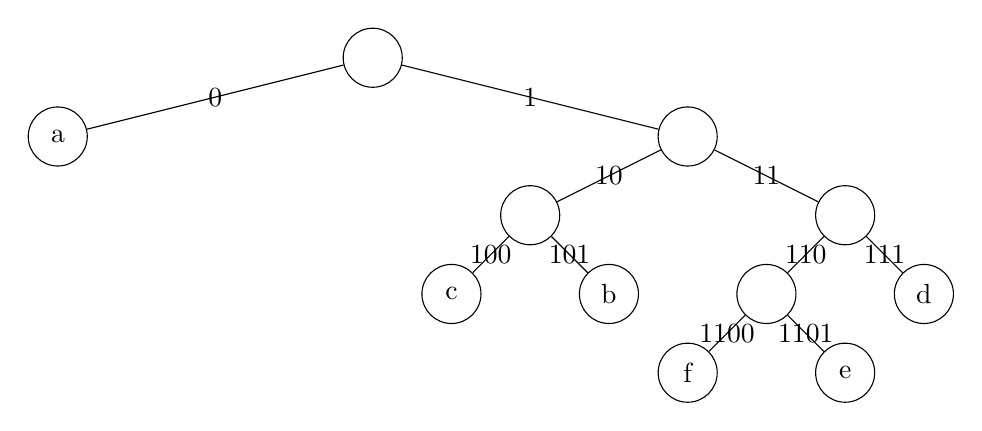
\begin{tikzpicture}[scale=0.5]
                    \node[draw, circle, minimum size=0.75cm] (root) at (16, 0) {};
                    \node[draw, circle, minimum size=0.75cm] (a) at (8, -2) {a};
                    \node[draw, circle, minimum size=0.75cm] (n1) at (24, -2) {};
                    \node[draw, circle, minimum size=0.75cm] (n2) at (20, -4) {};
                    \node[draw, circle, minimum size=0.75cm] (b) at (22, -6) {b};
                    \node[draw, circle, minimum size=0.75cm] (c) at (18, -6) {c};
                    \node[draw, circle, minimum size=0.75cm] (n3) at (28, -4) {};
                    \node[draw, circle, minimum size=0.75cm] (d) at (30, -6) {d};
                    \node[draw, circle, minimum size=0.75cm] (n4) at (26, -6) {};
                    \node[draw, circle, minimum size=0.75cm] (e) at (28, -8) {e};
                    \node[draw, circle, minimum size=0.75cm] (f) at (24, -8) {f};
                    % 
                    \draw (root) to node {0} (a);
                    \draw (root) to node {1} (n1);
                    \draw (n1) to node {10} (n2);
                    \draw (n1) to node {11} (n3);
                    \draw (n2) to node {101} (b);
                    \draw (n2) to node {100} (c);
                    \draw (n3) to node {111} (d);
                    \draw (n3) to node {110} (n4);
                    \draw (n4) to node {1101} (e);
                    \draw (n4) to node {1100} (f);
                \end{tikzpicture}
                \caption{Albero di Huffman per la codifica \texttt{Codifica 2}}
                \label{fig:huffman}
            \end{figure}
            La codifica di un carattere è data dal percorso per arrivare alla foglia corrispondente, ad esempio la codifica del carattere \texttt{a} è $0$, la codifica del carattere \texttt{b} è $101$, e così via.\newline
            Questo ci fa capire che per decodificare un carattere dall'albero dobbiamo seguire il percorso dall'alto verso il basso, se il bit letto è $0$ andiamo a sinistra, se è $1$ andiamo a destra, e quando arriviamo ad una foglia abbiamo decodificato il carattere e passiamo al carattere successivo.
        \subsubsection{Definizioni formali}
            Dato un file $F$ composto da $n$ caratteri, e un alfabeto $\sum$ di $m$ caratteri, inoltre siano:
            \begin{itemize}
                \item $T$ un albero binario di profondità $d$ e con $m$ foglie
                \item Per ogni $c \in \sum$, sia $d_T(c)$ la profondità della foglia $c$ nell'albero $T$
                \item Il codice per il carattere $c$ richiede $d_T(c)$ bit
                \item $f[c]$ il numero di occorrenze del carattere $c$ nel file $F$
            \end{itemize}
            Allora la dimensione della codifica del file $F$ è:
            $$
                C(F,T) = \sum_{c\in \sum} f[c] \cdot d_T(c)
            $$
            \paragraph{Principio del codice di Huffman} Il principio sul quale si basa l'algoritmo di Huffman è il seguente:
            \begin{itemize}
                \item Minimizzare la lunghezza dei caratteri più frequenti
                \item Assegnare ai caratteri meno frequenti codici più lunghi
            \end{itemize}
            inoltre ogni file ha la sua codifica che viene creata in base alla frequenza dei caratteri, e quindi non esiste una codifica ottima per tutti i file, ma solo per un certo file.
            \paragraph{Algoritmo} Si prende una sequenza di caratteri ai quali è associata la frequenza, si rimuovono i due nodi con frequenze minori ($f_x, f_y$), si crea un nuovo nodo con frequenza $f_x + f_y$ e con etichetta $-$, si collegano i due nodi rimossi al nuovo nodo, e si ripete il processo fino a quando non rimane un solo nodo, che sarà la radice dell'albero di Huffman.
            \paragraph{Implementazione}
                Di seguito l'implementazione dell'algoritmo di Huffman, che utilizza una coda di priorità per rimuovere i nodi con frequenza minima:
                \begin{algorithm}[H]
                    \caption{\Tree \textsc{huffman}(\Int[] $c$, \Int[] $f$, \Int $n$)}
                    \begin{algorithmic}
                        \State \PriorityQueue $Q \gets \New \PriorityQueue$ \Comment{Coda di priorità}
                        \For{\Int $i \gets 1$ \To $n$}
                            \State $Q.\Call{insert}(\Tree(c[i], f[i]), f[i])$
                        \EndFor
                        \For{\Int $i \gets 1$ \To $n-1$}
                            \State $z_1 \gets Q.\Call{deleteMin}()$
                            \State $z_2 \gets Q.\Call{deleteMin}()$
                            \State $z \gets \Tree(\Nil, z_1.f + z_2.f)$ \Comment{Creazione del nodo padre}
                            \State $z.left \gets z_1$
                            \State $z.right \gets z_2$
                            \State $Q.\Call{insert}(z, z.f)$
                        \EndFor
                    \end{algorithmic}
                \end{algorithm}
            \paragraph{Dimostrazione di correttezza} 
                La correttezza dell'algoritmo di Huffman è garantita dal fatto che, ad ogni iterazione, vengono rimossi i due nodi con frequenza minima, e quindi la codifica risultante sarà ottima. Inoltre, l'uso della coda di priorità garantisce che l'algoritmo abbia una complessità $O(n \log n)$. In questo caso la scelta \textit{greedy} consiste nel rimuovere i due nodi con frequenza minima e creare un nuovo nodo con frequenza $f_x + f_y$, in modo da minimizzare la lunghezza dei caratteri più frequenti. La tesi del teorema è che: esiste un codice prefisso ottimo per $\sum$ in cui $x,y$ hanno la stessa profondità massima e i loro codici differiscono per l'ultimo bit.
                \begin{proof}
                    $[\text{Omessa}]$
                \end{proof}
    \subsection{Albero di copertura di peso minimo}
        Il problema dell'albero di copertura di peso minimo è un problema di ottimizzazione combinatoria, in cui si cerca di trovare un albero di copertura di un grafo pesato che minimizzi il peso totale degli archi. (e.g. ottimizzazione di una rete di telecomunicazioni)
        \paragraph{Definizione} 
            Sia in input al problema $G=(V,E)$ un grafo pesato, non orientato, connesso, e sia $w: V\times V \rightarrow \mathbb{R}$ una funzione di peso definita sugli archi del grafo tale che se $(u,v) \in E$ allora $w(u,v)$ è il peso dell'arco $(u,v)$, e $w(u,v) = \infty$ se $(u,v) \notin E$. L'obiettivo è trovare un sotto-grafo $T$ di $G$ tale che:
            \begin{itemize}
                \item $T$ è un albero
                \item $T$ contiene tutti i vertici di $G$
                \item Il peso totale degli archi di $T$ è minimo
                \item $T$ è un albero di copertura di $G$
                \item $E_T \subseteq E$
            \end{itemize}
            Non esiste uno ed un solo albero di copertura di peso minimo, ma esistono più alberi di copertura di peso minimo, e quindi non è possibile determinare un albero di copertura di peso minimo in modo univoco.
        \subsubsection{Algoritmo generico}
            Come idea generale vogliamo prendere tutti gli ``archi sicuri'' ovvero quelli archi $(u,v)$ tali per cui $A\cap \{(u,v)\}$ è un sotto insieme di un qualsiasi albero di copertura minimo del grafo $G$. 
            \begin{algorithm}[H]
                \caption{\Set \textsc{mst-generico}(\Graph $G$, \Int[] $w$)}
                \begin{algorithmic}
                    \State \Set $A \gets \emptyset$
                    \While{$A$ non forma un albero di copertura}
                        \State trova un arco $(u,v)$ sicuro
                        \State $A \gets A \cup \{(u,v)\}$
                    \EndWhile
                    \State \Return $A$
                \end{algorithmic}
            \end{algorithm}
            